\section{What is a Graph}

\begin{problem}
	As in the text book.
\end{problem}
\begin{solution}
	$ k_{1,1} $ is the only complete bipartite graph that is also complete.
\end{solution}

\begin{problem}
	As in the textbook.
\end{problem}
\begin{solution}
	The adjacency matrices are:
	\[ A_1 = \begin{pmatrix}
		0 & 1 & 0 \\
		1 & 0 & 1 \\
		0 & 1 & 0
	\end{pmatrix},\qquad
	A_2 = \begin{pmatrix}
		0 & 1 & 1 \\
		1 & 0 & 0 \\
		1 & 0 & 0
	\end{pmatrix}, \qquad 
	A_3 = \begin{pmatrix}
		0 & 0 & 1 \\
		0 & 0 & 1 \\
		1 & 1 & 0
	\end{pmatrix}.
	 \]
	And the corresponding incidence matrices are:
	\[ 
	M_1 = \begin{pmatrix}
		1 & 0 \\
		1 & 1 \\
		0 & 1
	\end{pmatrix}, \qquad
	M_2 = \begin{pmatrix}
		1 & 1 \\
		1 & 0 \\
		0 & 1 
	\end{pmatrix}, \qquad 
	M_3 = \begin{pmatrix}
		1 & 0 \\
		0 & 1 \\
		1 & 1
	\end{pmatrix}
	 \]
	 
	An adjacency matrix for a path with six vertices is:
	\[ A = \begin{pmatrix}
		0 & 1 & 0 & 0 & 0 & 0 \\
		1 & 0 & 1 & 0 & 0 & 0 \\
		0 & 1 & 0 & 1 & 0 & 0 \\
		0 & 0 & 1 & 0 & 1 & 0 \\
		0 & 0 & 0 & 1 & 0 & 1 \\
		0 & 0 & 0 & 0 & 1 & 0 \\
	\end{pmatrix}.
	 \]
	And an adjacency matrix for a cycle with six vertices is:
	\[ A = \begin{pmatrix}
		0 & 1 & 0 & 0 & 0 & 1 \\
		1 & 0 & 1 & 0 & 0 & 0 \\
		0 & 1 & 0 & 1 & 0 & 0 \\
		0 & 0 & 1 & 0 & 1 & 0 \\
		0 & 0 & 0 & 1 & 0 & 1 \\
		1 & 0 & 0 & 0 & 1 & 0 \\
	\end{pmatrix}.
	\]
\end{solution}

\begin{problem}
	As in the textbook.
\end{problem}
\begin{solution}
	An adjacency matrix for $ K_{n,m} $ can be written as
	\[
	A =
	\begin{pmatrix}
		0_{n \times n} & I_{n \times m} \\
		I_{m \times n} & 0_{m \times m},
	\end{pmatrix}
	\]
	for which we have ordered the vertices as $ (v_1,v_2,\cdots,v_n,v_{n+1},\cdots,v_{n+m}), $
	where $ v_1,\cdots,v_m $ all belong to one partide, and $ v_{n+1},\cdots,v_{n+m} $ all belong to the other partide.
\end{solution}


\begin{problem}
	From the definition of isomorphism, prove that $ G\cong H $ if and only if $ \overline{G} \cong \overline{H} $.
\end{problem}
\begin{solution}
	For the first direction, assume $ G \cong H $. We want to show $ \overline{G} \cong \overline{H} $. Since $ G \cong H $, $ \exists f: V(G) \to V(H) $ such that $ ab \in E(G) $ iff $ f(a)f(b) \in E(H) $. Let $ xy \in E(\overline{G}) $. Then $ xy \notin E(G) $. Using the fact that $ f $ is isomorphism, $ f(x)f(y) \notin E(H) $. So $ f(x)f(y) \in E(\overline{H}) $. Furthermore, let $ uv \notin E(\overline{G}) $. So $ uv\in E(G) \biImp f(u)f(v) \in E(H) \biImp f(u)f(v)\notin E(\overline{H})$. So $ f $ is an isomorphism between $ \overline{G} $ and $ \overline{H} $. The other direction of the proof can be shown similarly.
\end{solution}


\begin{problem}
	Prove or disprove. If every vertex of a simple graph $ G $ has degree 2, then $ G $ is a cycle.
\end{problem}
\begin{solution}
	Not true. Two copies of $ K_3 $ is a counterexample.
\end{solution}

\begin{problem}
	As in the textbook.
\end{problem}
\begin{solution}
	Consider the following decomposition.
	\begin{figure}[h!]
	\centering
	
	
	
	\tikzset{every picture/.style={line width=0.75pt}} %set default line width to 0.75pt        
	
	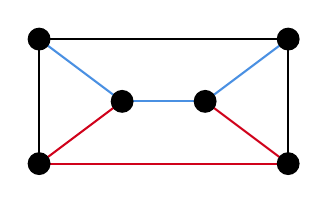
\begin{tikzpicture}[x=0.75pt,y=0.75pt,yscale=-1,xscale=1]
		%uncomment if require: \path (0,300); %set diagram left start at 0, and has height of 300
		
		%Straight Lines [id:da29435505087653746] 
		\draw [color={rgb, 255:red, 208; green, 2; blue, 27 }  ,draw opacity=1 ][fill={rgb, 255:red, 74; green, 144; blue, 226 }  ,fill opacity=1 ]   (195,105) -- (235,75) ;
		%Straight Lines [id:da15130033487443384] 
		\draw [color={rgb, 255:red, 208; green, 2; blue, 27 }  ,draw opacity=1 ][fill={rgb, 255:red, 74; green, 144; blue, 226 }  ,fill opacity=1 ]   (195,105) -- (315,105) ;
		%Straight Lines [id:da9313777412496024] 
		\draw [color={rgb, 255:red, 208; green, 2; blue, 27 }  ,draw opacity=1 ][fill={rgb, 255:red, 74; green, 144; blue, 226 }  ,fill opacity=1 ]   (275,75) -- (315,105) ;
		%Straight Lines [id:da979754963449776] 
		\draw [color={rgb, 255:red, 74; green, 144; blue, 226 }  ,draw opacity=1 ][fill={rgb, 255:red, 74; green, 144; blue, 226 }  ,fill opacity=1 ]   (275,75) -- (235,75) ;
		%Straight Lines [id:da11218419538778379] 
		\draw [color={rgb, 255:red, 74; green, 144; blue, 226 }  ,draw opacity=1 ][fill={rgb, 255:red, 74; green, 144; blue, 226 }  ,fill opacity=1 ]   (315,45) -- (275,75) ;
		%Straight Lines [id:da44553444033080924] 
		\draw [color={rgb, 255:red, 74; green, 144; blue, 226 }  ,draw opacity=1 ][fill={rgb, 255:red, 74; green, 144; blue, 226 }  ,fill opacity=1 ]   (235,75) -- (195,45) ;
		%Shape: Circle [id:dp5069495015265886] 
		\draw  [fill={rgb, 255:red, 0; green, 0; blue, 0 }  ,fill opacity=1 ] (190,45) .. controls (190,42.24) and (192.24,40) .. (195,40) .. controls (197.76,40) and (200,42.24) .. (200,45) .. controls (200,47.76) and (197.76,50) .. (195,50) .. controls (192.24,50) and (190,47.76) .. (190,45) -- cycle ;
		%Shape: Circle [id:dp25021666713761814] 
		\draw  [fill={rgb, 255:red, 0; green, 0; blue, 0 }  ,fill opacity=1 ] (190,105) .. controls (190,102.24) and (192.24,100) .. (195,100) .. controls (197.76,100) and (200,102.24) .. (200,105) .. controls (200,107.76) and (197.76,110) .. (195,110) .. controls (192.24,110) and (190,107.76) .. (190,105) -- cycle ;
		%Shape: Circle [id:dp606959925111063] 
		\draw  [fill={rgb, 255:red, 0; green, 0; blue, 0 }  ,fill opacity=1 ] (310,45) .. controls (310,42.24) and (312.24,40) .. (315,40) .. controls (317.76,40) and (320,42.24) .. (320,45) .. controls (320,47.76) and (317.76,50) .. (315,50) .. controls (312.24,50) and (310,47.76) .. (310,45) -- cycle ;
		%Shape: Circle [id:dp7417260861337834] 
		\draw  [fill={rgb, 255:red, 0; green, 0; blue, 0 }  ,fill opacity=1 ] (310,105) .. controls (310,102.24) and (312.24,100) .. (315,100) .. controls (317.76,100) and (320,102.24) .. (320,105) .. controls (320,107.76) and (317.76,110) .. (315,110) .. controls (312.24,110) and (310,107.76) .. (310,105) -- cycle ;
		%Shape: Circle [id:dp47320961285111385] 
		\draw  [fill={rgb, 255:red, 0; green, 0; blue, 0 }  ,fill opacity=1 ] (230,75) .. controls (230,72.24) and (232.24,70) .. (235,70) .. controls (237.76,70) and (240,72.24) .. (240,75) .. controls (240,77.76) and (237.76,80) .. (235,80) .. controls (232.24,80) and (230,77.76) .. (230,75) -- cycle ;
		%Shape: Circle [id:dp9913663913060298] 
		\draw  [fill={rgb, 255:red, 0; green, 0; blue, 0 }  ,fill opacity=1 ] (270,75) .. controls (270,72.24) and (272.24,70) .. (275,70) .. controls (277.76,70) and (280,72.24) .. (280,75) .. controls (280,77.76) and (277.76,80) .. (275,80) .. controls (272.24,80) and (270,77.76) .. (270,75) -- cycle ;
		%Straight Lines [id:da7053823784402796] 
		\draw    (195,45) -- (315,45) ;
		%Straight Lines [id:da848171725259851] 
		\draw    (315,45) -- (315,105) ;
		%Straight Lines [id:da2625430487899586] 
		\draw    (195,105) -- (195,45) ;
		
		
		
		
	\end{tikzpicture}
\end{figure}
\end{solution}

\begin{problem}
	Prove that a graph with more than six vertices of off degree can not be decomposed into three paths.
\end{problem}











